\vspace{24pt}
\chapter{Координатные детекторы на основе GEM}
\label{sec:coor_GEM}
\section{Общие принципы работы газовых координатных детекторов}
Измерения координат частиц проводятся с помощью довольно широкого спектра устройств, использующих различные физические принципы в основе своей работы. В отдельную группу стоит выделить газовые координатные детекторы. В основу их работы легло явление ионизации атомов газа первичной заряженной частицей. Если зарегистрировать первичную ионизацию -- заряд, образовавшийся после пролета частицы через чувствительную область детектора, то можно восстановить её координаты. Основная проблема заключается в том, что для первичной частицы ионизация составляет по порядку величины $10 \div 100$ электрон--ионных пар на 1 см трека. Регистрация таких малых зарядов представляется проблематичной. Поэтому в детекторной технике используются различные усиливающие устройства, которые позволяют увеличивать количество заряда до значений, при которых его можно зарегистрировать современными зарядочувствительными устройствами \cite{grupen}.
\par При создании детектора для установки <<Лазерный поляриметр>> были выдвинуты требования, которые позволили определить тип используемой усилительной системы и общую схему детектора. Наиболее важные из них: 
\begin{itemize}
	\item регистрация координат фотонов
	\item достаточное для достоверного наблюдения эффекта порядка 0.1\,мм пространственное разрешение 
	\item возможность одновременного детектирования нескольких событий 
	\item компактные размеры, простота и надежность конструкции
\end{itemize}
Регистрация фотонов с энергиями $\sim1\GeV$ обычно производится посредством их конверсии в электрон--позитронные пары и последующей регистрации уже заряженных частиц. После рассмотрения возможных схем, удовлетворяющих данным требованиям, было решено остановиться на т.н. микроструктурных детекторах, как на наиболее простых и, в то же время, обеспечивающих требуемое пространственное разрешение. Это достаточно новый тип детекторов \cite{sauli}, однако в ИЯФ СО РАН накоплен сравнительно большой опыт по работе с ними.
\section{Газовые микроструктурные детекторы}
Идея использования микроструктурных газовых координатных детекторов получила развитие в CERN в 1980--х г. Многие детекторы данного типа имеют схожий принцип работы: с помощью проводников определенной формы в газовой среде создаются локальные области с высокой напряженностью поля. При попадании в них, заряженная частица на длине свободного пробега приобретает энергию, большую, чем энергия ионизации атомов газовой смеси. 
\begin{figure}[h]
	\centering
	\begin{subfigure}{.45\textwidth}
		\centering
		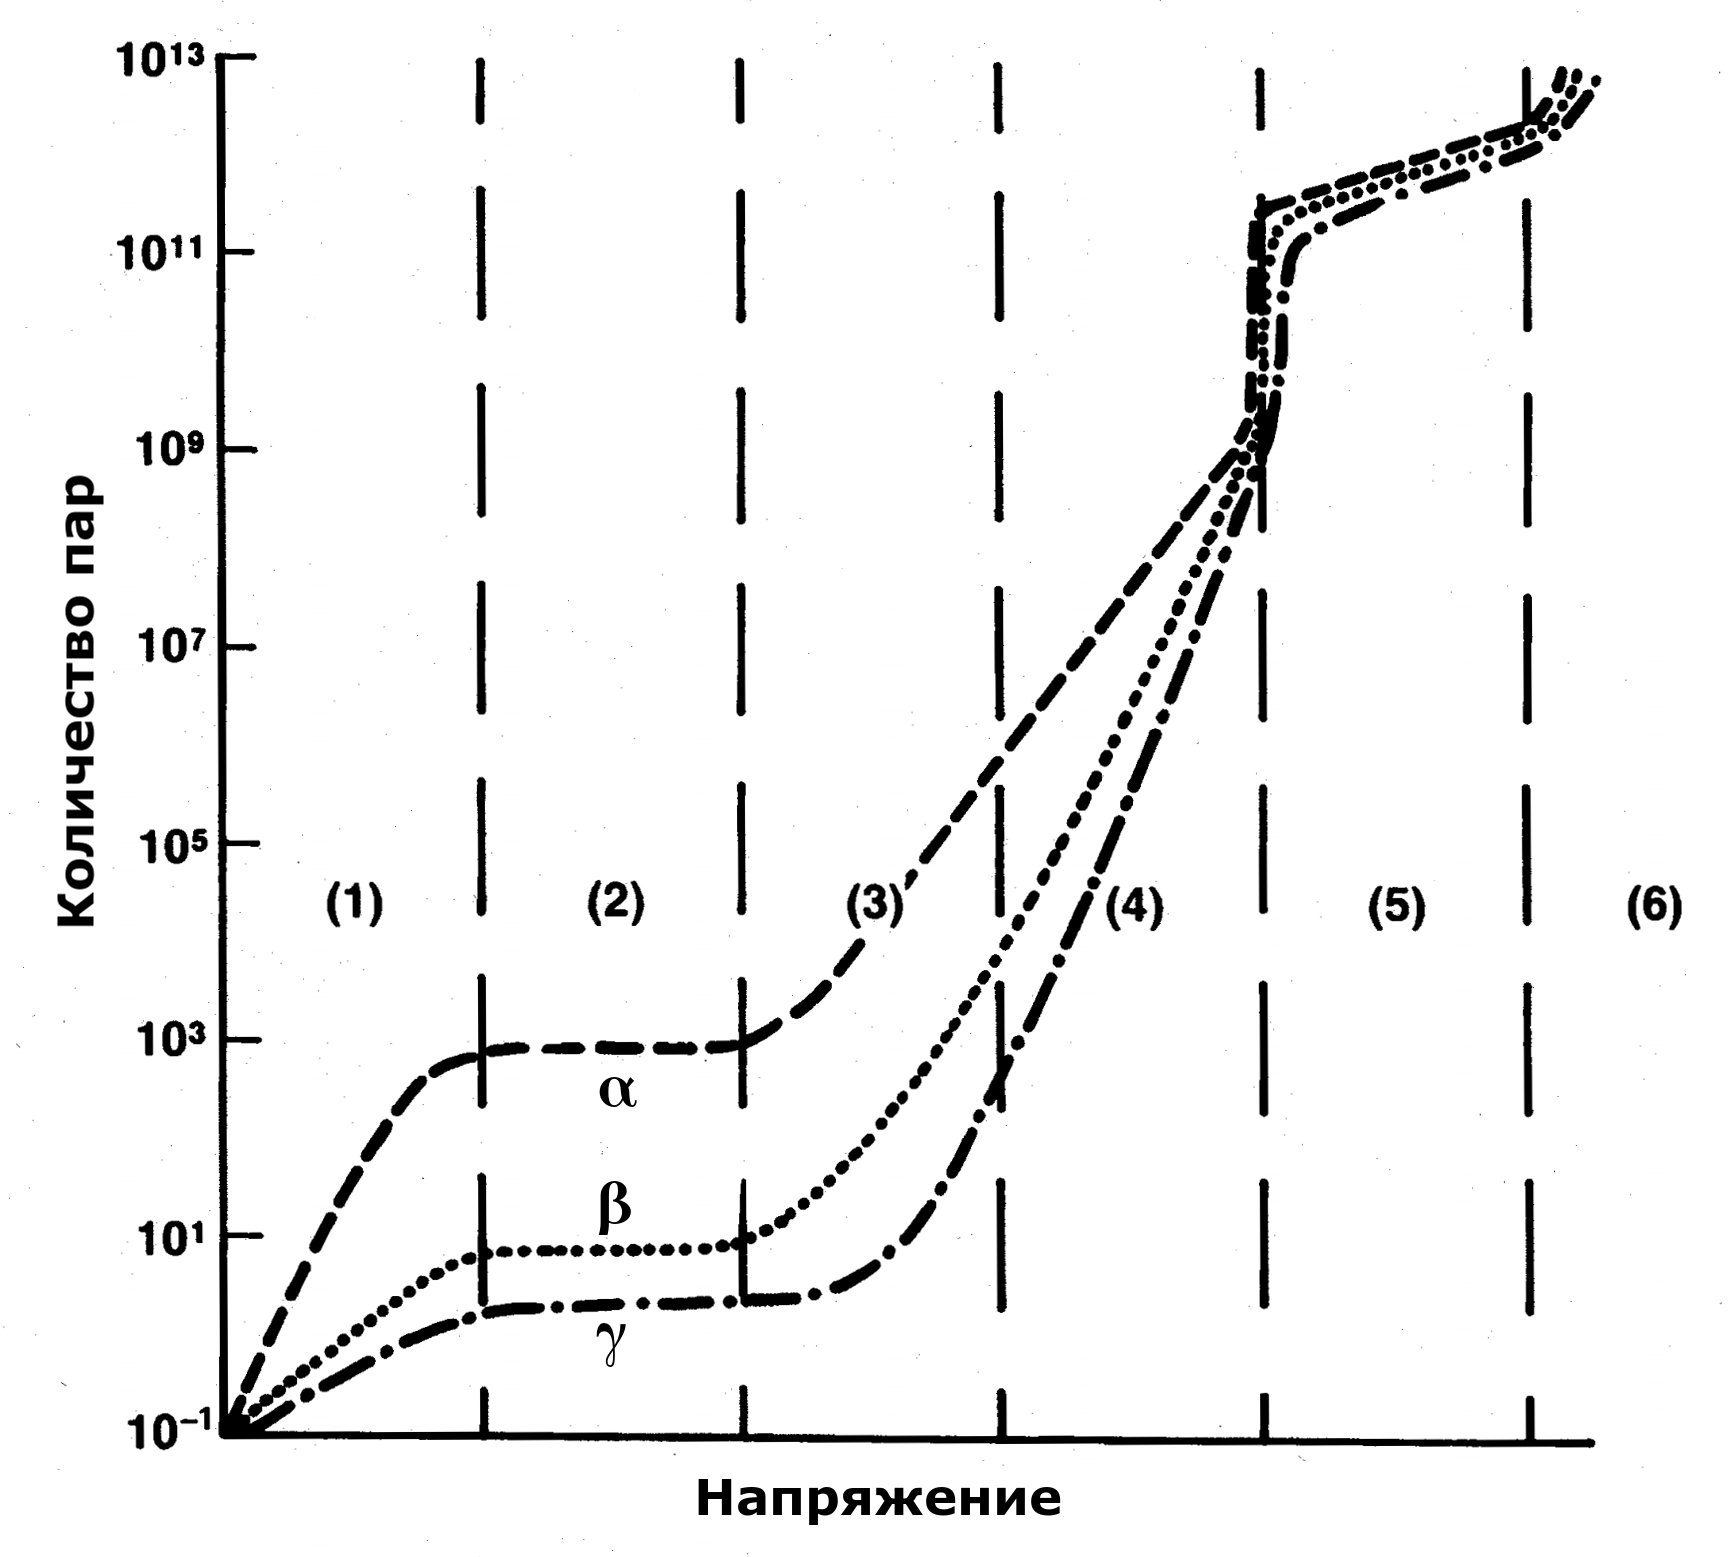
\includegraphics[width=0.9\linewidth]{img/Gas_discharge_gr.png}
		\caption{Зависимость удельного количества электрон-ионных пар от напряжения, приложенного электродам в газовом промежутке. Количество ионизации различно для $\alpha,\beta$ и $\gamma$--частиц.}
	\end{subfigure}
	\hspace{20pt}
	\begin{subfigure}{.45\textwidth}
		\centering
		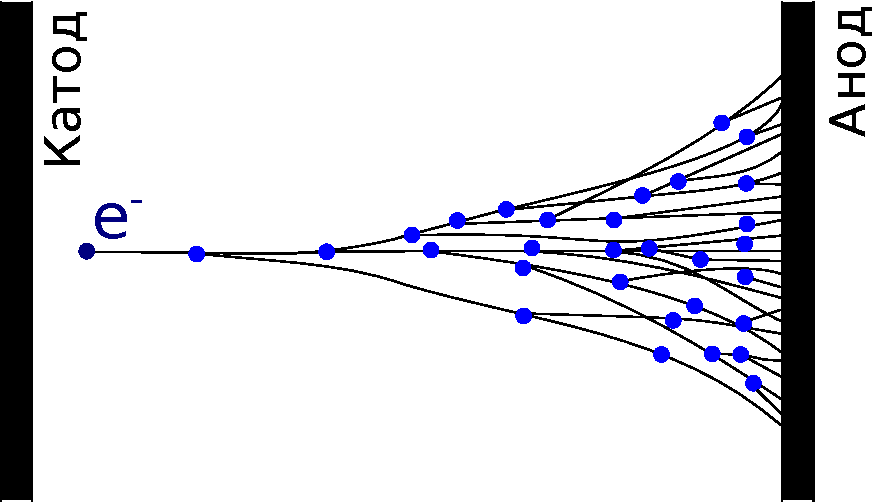
\includegraphics[width=1\linewidth]{img/Electron_avalanche.pdf}
		\caption{Образование электронной лавины. В пропорциональном режиме количество вторичных электронов экспоненциально растет с координатой, вдоль которой движется частица. Полное их число пропорционально первичной ионизации}
	\end{subfigure}%
	\caption{Режимы работы газовых детекторов определяются напряженностью электрического поля в газовом промежутке, которое зависит от напряжения на электродах детектора и его геометрии. Микроструктурные детекторы работают в пропорциональной области (3)}
	\label{fig:gas_discharge}
\end{figure}
 Поэтому становится возможным образование электрон-ионных пар. Из-за того, что подвижность ионов почти на 3 порядка меньше подвижности электронов, основной вклад в эффект объясняется движением электронов. Более того, количество заряженных частиц экспоненциально растет, но электрического пробоя не происходит. Это объясняется определенной геометрией электродов, а так же экранировкой внешнего поля полем свободных зарядов. Т.к. микроструктурные детекторы работают в пропорциональном режиме, то суммарное количество заряда пропорционально первичной ионизации.
 \par Рассмотрим подробнее один из видов микроструктурных детекторов -- газовые электронные умножители, которые было решено применены в конструкции  Они были впервые созданы группой Ф. Саули в CERN в 1997 г. и на данный момент активно исследуются и применяются в современных детектирующих системах. 
 \begin{figure}[h]
 	\centering
 	\begin{minipage}{.45\textwidth}
 	\centering
 	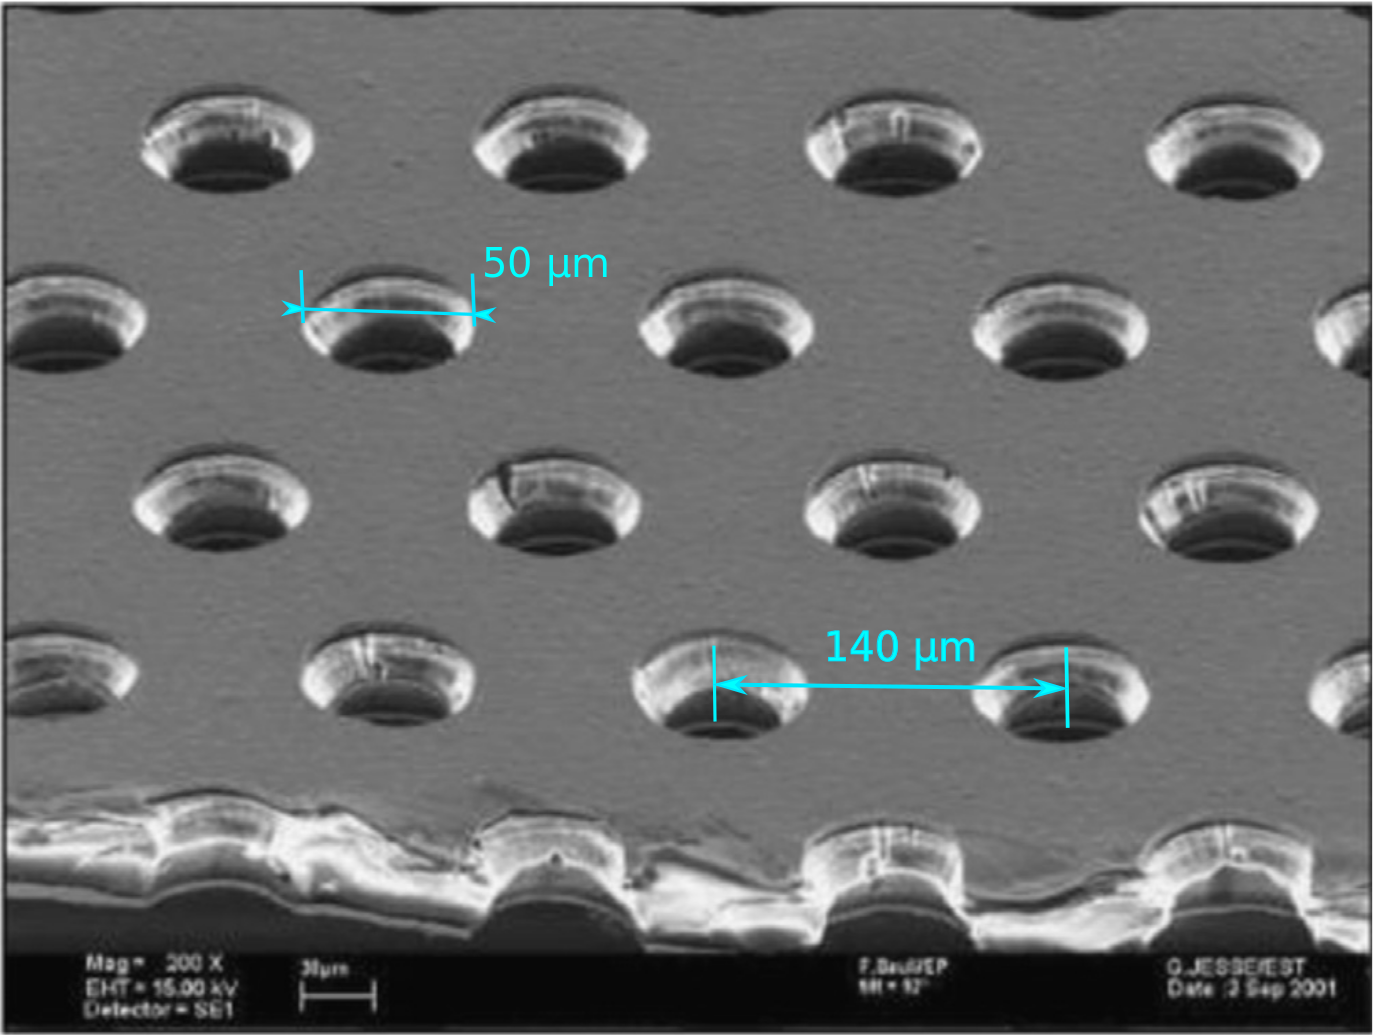
\includegraphics[width=1\linewidth]{img/GEM_microphoto.png}
 	\caption{Микрофотография GEM. Видны последовательные ряды отверстий конической формы, протравленных в медном электроде и полиимидной пленке.}
 	\end{minipage}
 	\hspace{20pt}
 	\begin{minipage}{.45\textwidth}
 			\centering
 		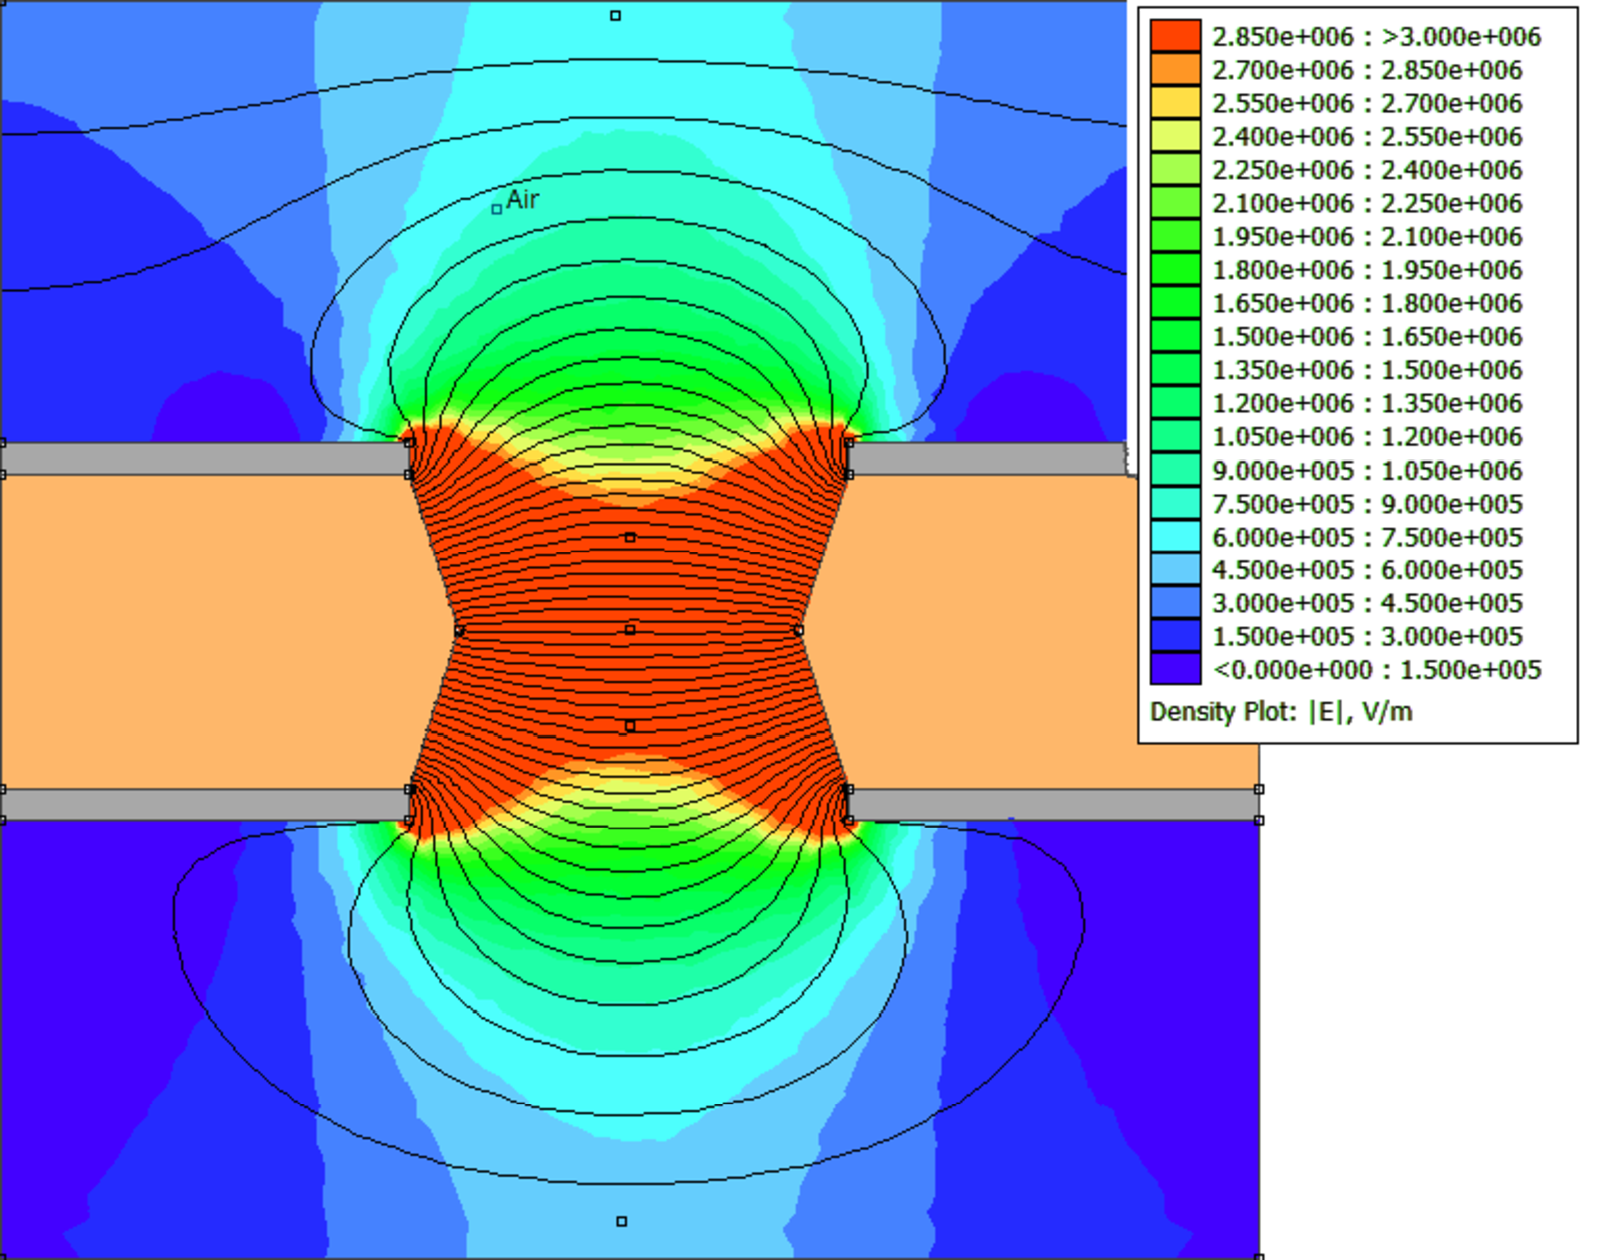
\includegraphics[width=1\linewidth]{img/GEM_field.pdf}
 		\caption{Моделирование распределения электрического поля в отверстии GEM методом конечных элементов.}
 	\end{minipage}
 \end{figure}
 Газовый электронный умножитель представляет собой полиимидную плёнку толщиной 50\,мкм, покрытую с двух сторон слоями меди, толщиной 5\,мкм. В слоях меди и полиимида протравливаются отверстия размером 50\,мкм с шагом 140\,мкм. Такая конструкция позволяет точно (до 100\,нм) выдерживать размеры отверстий и расстояние между электродами, а значит и величину электрического поля в отверстиях. Этот параметр напрямую влияет на коэффициент усиления и прозрачность GEM, а в конечном итоге на эффективность регистрации и надежность детектора.
 \par Наиболее простая конструкция детектора на основе  GEM состоит из катодного электрода, в качестве которого обычно применяют фольгированный полимид, анодного электрода (или группы электродов в случае координатного детектора) и GEM, расположенного между ними.
 \begin{figure}[h]
	\centering
	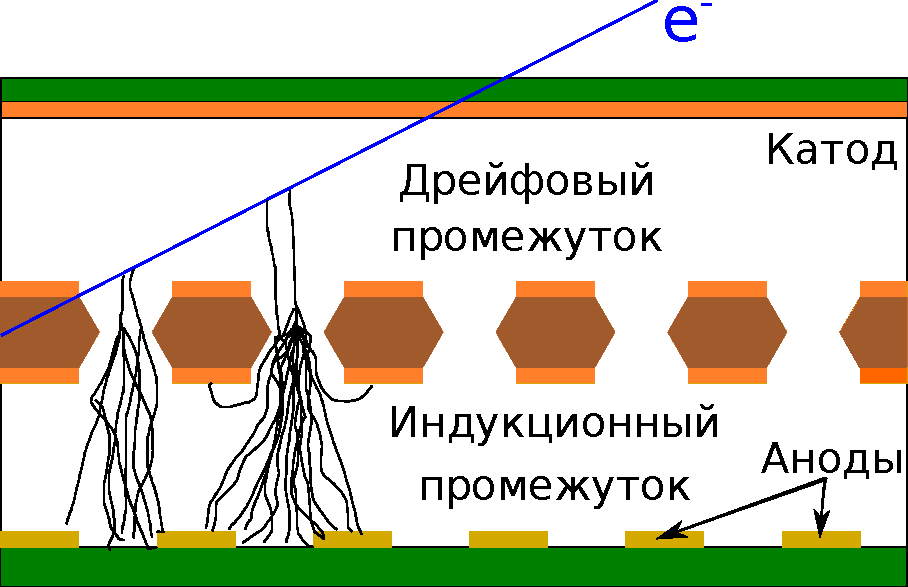
\includegraphics[height = 4 cm, width= 6cm]{img/GEM_scheme.pdf}
	\caption{Схема детектора на основе GEM. Первичная частица вызывает ионизацию в дрейфовом промежутке, которая, проходя через GEM--электрод создает электронные лавины, регистрируемые считывающей структурой.}
	\label{fig:single} 	
 \end{figure}
  следующий: к медным электродом прикладывается напряжение порядка 300 В, и в отверстиях создается поле порядка 1 МВ/м. Первичная ионизирующая частица проникает в дрейфовый промежуток, где ионизирует атомы газовой смеси. Электроны ионизации дрейфуют к GEM--электроду, в котором образуются электронные лавины. Вторичная ионизация попадает в индукционный промежуток и регистрируется анодами детектора.
 \par В случае когда требуется обеспечить большие коэффициенты усиления или высокую эффективность регистрации, электроды GEM можно размещать последовательно, формируя дополнительные транспортные промежутки. Так можно достичь коэффициентов усиления вплоть до $10^7$ \cite{sauli}. Ограничением на максимальное количество заряда, образуемое в электронной лавине, то есть на максимальный коэффициент усиления является т.н. предел Рейтера, который равняется приблизительно $Q_{max} = 10^6\div10^7~e^-$. При достижении зарядом лавины данного значения вероятность электрического пробоя резко возрастает, поэтому следует выбирать оптимум по параметрам детектора между усилением схемы и вероятностью возникновения пробоя. 
  
 



